\section{Customizing PFunc} 
\label{sec:custom}

The novelty of PFunc is that many of its runtime components can be configured
and/or extended using generic programming techniques.
%
PFunc's policy-based design allows users to customize its
user-provided components, and indirectly, the generated components as well
through three key features: \emph{scheduling policy}, \emph{compare}, and
\emph{work}.
%
These features directly influence the selection and composition of the
different components that are used in PFunc at runtime.
%
Furthermore, underlying the features are different concepts, which the values
chosen for these features must model.
%
Figure~\ref{fig:custom} depicts the role played by each feature in the
selection of the different components of PFunc.
%
To assist application parallelization ``out-of-the-box'', PFunc provides a 
number of built-in choices for each feature.
%
In this section, we explore the scheduling policy, compare, and work features,
their related concepts, and their built-in values in detail.

There are many different ways of representing concepts and their models.
%
In this section, all the concepts and their models are defined using the syntax
of \ConceptCpp{}, a proposal to add direct support for concepts into the \Cpp{}
language.
%
An important reason for choosing \ConceptCpp{} is that we are able to test the
correctness of our concepts and their models using the reference ConceptGCC
compiler implementation.\footnote{ConceptGCC does not handle templated
associated functions; such functions had to be commented out.}
%
For the sake of brevity, the concepts defined in PFunc make use of other
\emph{external concepts}; these are summarized in
Table~\ref{tbl:external_concepts}.
%
As can be seen, PFunc makes use of concepts from two sources: the \ConceptCpp{}
proposal and the Silicon Graphics International's (SGI) version of the STL.

\begin{figure}
\centering
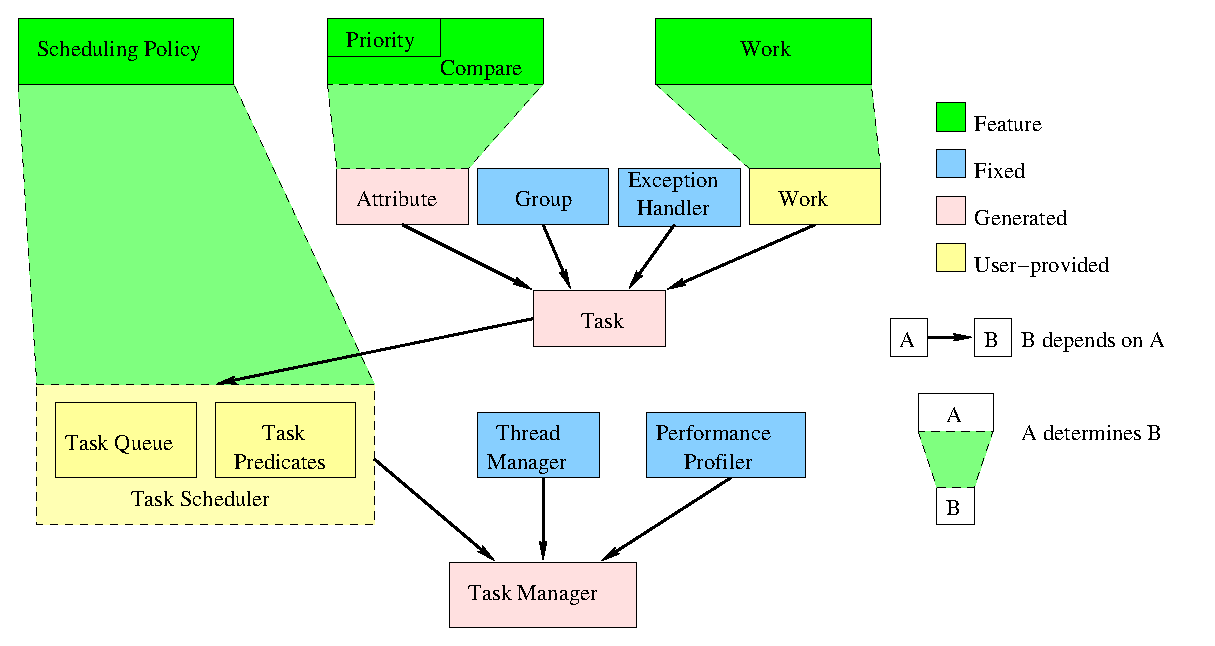
\includegraphics[width=1.0\textwidth]{figs/custom}
\caption{An overview of the configuration diagram for PFunc. PFunc provides
three features (colored green; scheduling policy, compare, and work) that can
be used to generate a variety of library instance descriptions.  Components
colored yellow are user-provided and are either selected from a built-in list
or are implemented by users. Components colored pink are generated from values
given to the three features. Components colored blue are fixed, and hence, are 
not configurable at compile time.}
\label{fig:custom}
\end{figure}

\begin{table}[t]
\centering
\tablefont
\begin{tabular}{|c|c|l|}
\hline
Concept name & Parameters & Description \\
\hline
\concept{Copy Constructible} & \code{T} & Requires the ability to create and destroy copies of objects of type \code{T}. \\
\hline
\concept{Copy Assignable} & \code{T} & Requires the ability to assign values to objects of type \code{T}. \\
\hline
\concept{Default Constructible} & \code{T} & Requires the existence of an accessible default constructor for type \code{T}.\\
\hline
\concept{Same Type} & \code{T1}, \code{T2} & Requires that both \code{T1} and \code{T2} have the exact same type. \\
\hline
\concept{CallableN} & \code{F}, \code{T1}, ..., \code{TN} & Represents a family of concepts (\concept{Callable0}, \concept{Callable1}, ..., \concept{CallableN}). \\
                    & & Requires that \code{F} be callable with given arguments of type \code{T1}, \code{T2}, ... \code{TN}. \\
                    & & Requires that \code{result\_type} be a nested type. \\
\hline
\concept{Adaptable Binary Function} & \code{F}, \code{T1}, \code{T2} & Requires that \code{F} be callable with arguments of type \code{T1} and {T2}. \\
                          & & Requires that \code{first\_argument\_type} and \code{second\_argument\_type} be nested types. \\
                          & & Requires that \code{result\_type} be a nested type. \\
\hline
\end{tabular}
\caption{A summary of all the external concepts that are used in PFunc. All the
listed concepts (other than the \concept{Adaptable Binary Function} concept)
are defined in \ConceptCpp{}. The \concept{Binary Function} concept is
defined in the Silicon Graphics International's (SGI) STL technical
archives.}
\label{tbl:external_concepts}
\end{table}

\subsection{Generator}
\label{subsec:lib_instance}

Like the STL, PFunc is a library template ; in order to use it, users are first
required to generate a concrete library instance description by providing
appropriate values to the three customizable features.
%
These features not only represent the values for the user-provided components,
but also are used to create concrete instances of the generated components. 
%
To facilitate this process, PFunc provides \code{pfunc::generator}, a templated
generator class that accepts three template parameters, each of which represent
a value of a particular feature.
%
The definition of \code{pfunc::generator} is given below:

\begin{lstlisting}[columns=flexible]
template <typename PolicyName, typename Compare, typename Work>
  requires SchedulingPolicy<PolicyName, pfunc::detail::task<Compare, Work> > &&
           AdaptableCallableN<Compare> &&
           Callable0<Work>
struct pfunc::generator { 
  /* type definitions for user-provided and generated components */ 
};
\end{lstlisting}
 
As can be seen, each template parameter (feature) is constrained with
corresponding concept requirements.
%
First, \code{PolicyName} must be a model of the \concept{Scheduling Policy}
concept, defined in Section~\ref{subsec:scheduling_policy}.
%
This concept takes in an additional parameter, \code{TaskType} (represented 
by the template type \code{pfunc::detail::task<T,U>}) that must be a model of
the \concept{PFunc Task} concept defined in
Figure~\ref{fig:pfunc_task_concept}.
%
Second, \code{Compare} is constrained to be a model of one of the the
\concept{Adaptable CallableN} family of concepts, defined in
Section~\ref{subsec:compare}.
%
Finally, \code{Work} must be a model of the \concept{Callable0} concept,
defined in \ConceptCpp{}.

To make PFunc work ``out-of-the-box'', we provide \code{pfunc::use\_default}, a
special class that can be used as the default value of any feature.
%
Specialization of \code{pfunc::generator} for different positional combinations
of \code{pfunc::use\_default} is used to substitute appropriate built-in values
as defaults for each feature (\code{cilkS} for \code{PolicyName},
\code{std::less<int>} for \code{Compare}, and
\code{pfunc::detail::virtual\_functor} for \code{Work}).
%
Once the three template parameters are specified, the library instance
description is generated; this instance exposes the required PFunc components
(work, attribute, group, task, and task manager) as nested types, which are
required to parallelize user applications.

\subsection{Scheduling Policy}
\label{subsec:scheduling_policy}

The value given to this feature determines the scheduling policy that is
used in the generated library instance description; that is, it determines the
task queue and task predicate components.
%
PFunc offers four built-in values for this feature: \code{cilkS}, \code{prioS},
\code{lifoS}, and \code{fifoS}; in addition, users can define custom scheduling
polices.
%
Values given to the scheduling policy feature must model the
\concept{Scheduling Policy} concept, defined below.
%
\begin{lstlisting}
concept SchedulingPolicy <typename PolicyName, typename TaskType> {
  /* concept requirements */
  requires PFuncTask <TaskType>;
  @\halfline@
  /* associated types */
  typename task_queue_set;
  typename regular_predicate_pair;
  typename waiting_predicate_pair;
  typename group_predicate_pair;
  @\halfline@
  /* associated type requirements */
  requires TaskQueueSet <PolicyName, task_queue_set>;
  requires TaskPredicatePair <PolicyName, regular_predicate_pair>;
  requires SameType <TaskType*, regular_predicate_pair::value_type>;
  requires TaskPredicatePair <PolicyName, waiting_predicate_pair>;
  requires SameType <TaskType*, waiting_predicate_pair::value_type>;
  requires TaskPredicatePair <PolicyName, group_predicate_pair>;
  requires SameType <TaskType*, group_predicate_pair::value_type>;
}
\end{lstlisting}
%
The \concept{Scheduling Policy} concept takes two parameters: \code{PolicyName}
and \code{TaskType}.
%
\code{TaskType}, the second (additional) parameter, is required because it
influences the type of the components (task queue and task predicate) that
implement the scheduling policy.
%
Any type used as \code{TaskType} is required to model the \concept{PFunc Task}
concept defined in Figure~\ref{fig:pfunc_task_concept}.
%
In PFunc, the task is a generated component whose type is jointly determined by
the values of both the compare and work features; it is represented by the
template type \code{pfunc::detail::task<T,U>}.
%
Briefly, the \concept{PFunc Task} concept stipulates that any valid
\code{TaskType} must be a model of both \concept{Copy Constructible} and
\concept{Copy Assignable} concepts.
%
Furthermore, it is required to have \code{compare\_type} and \code{work\_type}
as associated types.
%
In turn, \code{compare\_type} is required to be a model of one of the concepts
in the \concept{Adaptable CallableN} family of concepts (see
Section~\ref{subsec:compare}) and \code{work\_type} is required to be a model
of the \concept{Callable0} concept (see Section~\ref{subsec:custom_work}).
%
Finally, \code{TaskType} must define the \func{TaskType::get\_compare}
associated function, which returns returns an object of type
\code{compare\_type} when it is invoked.
%
\begin{figure}
\begin{center}
\begin{minipage}{0.8\textwidth}
\begin{lstlisting}[frame=trbl]
concept PFuncTask <typename TaskType> {
  /* concept requirements */
  requires CopyConstructible <TaskType> && CopyAssignable <TaskType>;
  @\halfline@
  /* associated types */
  typename compare_type;
  typename work_type;
  @\halfline@
  /* associated type requirements */
  requires AdaptableCallableN<compare_type>;
  requires Callable0<work_type>;
  @\halfline@
  /* associate functions */
  compare_type TaskType::get_compare () const;
}
\end{lstlisting}
\end{minipage}
\end{center}
\caption{The concept definition of the \concept{PFunc Task} concept, which
governs type of the task objects in PFunc (of type \code{TaskType}.)}
\label{fig:pfunc_task_concept}
\end{figure}
%
Models of the \concept{Scheduling Policy} concept must define four
associated types: \code{task\_queue\_set}, \code{regular\_predicate\_pair},
\code{waiting\_predicate\_pair}, and \code{group\_predicate\_pair}.
%
Of these, the \code{task\_queue\_set} associated type represents the task queue
component and must be a model of the \concept{Task Queue Set} concept (defined
in Section~\ref{subsubsec:task_queue_set}).
%
The remaining three associated types together form the task predicate component
and must be models of the \concept{Task Predicate Pair} concept, which is
defined in Section~\ref{subsubsec:task_predicate}.

\subsubsection{Task Predicate Pair}
\label{subsubsec:task_predicate}
%
Every scheduling policy must define the three predicate pairs that form the
task predicate component; each pair must model the \concept{Task Predicate
Pair} concept, defined below.

\begin{lstlisting}
concept TaskPredicatePair <typename PolicyName, typename PredPair> {
  /* associated types */
  typename value_type;
  typename result_type;
  @\halfline@
  /* associated functions */
  PredPair::PredPair(value_type);
  result_type PredPair::own_pred(value_type);
  result_type PredPair::steal_pred(value_type);
}
\end{lstlisting}
% 
The \concept{Task Predicate Pair} concept takes two parameters:
\code{PolicyName} and \code{PredPair}. 
%
In other words, \concept{Task Predicate Pair} ensures that \code{PredPair} can
be used by the scheduling policy defined by \code{PolicyName}.
%
The \concept{Task Predicate Pair} concept defines two associated types: 
\code{value\_type} and \code{result\_type}, and three associated functions:
\func{PredPair::PredPair}, \func{own\_pred}, and \func{steal\_pred}.
%
Like the \code{PolicyName}, the \code{value\_type} associated type is used to 
ensure compatibility between the task predicate and task scheduling components.
%
At each scheduling point, the thread manager constructs a new \code{PredPair}
corresponding to the type of the scheduling point, and passes it as an argument
to the task queue component.
%
Therefore, the time required to construct a predicate pair directly adds to
the task scheduling overhead, and it is advisable to have \emph{light} task
predicates that can be constructed quickly.
%
New predicate pairs are constructed by invoking their respective initializing
constructors (\func{PredPair::PredPair}); at this time, these predicates are
passed a pointer to the task previously executed by the calling thread.
%
This (task) pointer contains information about the previously executed task's
attributes, which can be used by the task queue component to evaluate the
goodness of the candidate tasks when picking the next task to execute.
%
To evaluate the candidate tasks in the calling thread's own queue, the
\func{PredPair::own\_pred} associated function is used; else (when stealing),
the \func{PredPair::steal\_pred} associated function is used.

\subsubsection{Task Queue Set}
\label{subsubsec:task_queue_set}
%
For a policy to be a valid value of the scheduling policy feature, it must
define a task queue component. 
%
The task queue component is governed by the \concept{Task Queue Set} concept
defined below.

\begin{lstlisting}[columns=flexible]
concept TaskQueueSet <typename PolicyName, typename QueueSet> {
  /* associated types */
  typename value_type;
  typename queue_index_type;
  @\halfline@
  /* associated type requirements */
  requires PFuncTask <remove_pointer<value_type>::result_type>;
  requires CopyConstructible <queue_index_type> && 
           CopyAssignable <queue_index_type> &&
           DefaultConstructible <queue_index_type>;
  @\halfline@
  /* associated functions */
  QueueSet::QueueSet (unsigned int);
  void QueueSet::put (queue_index_type, const value_type&);
  template <typename PredPair>
  requires TaskPredicatePair<PredPair, PolicyName> &&
           SameType<TaskPredicatePair<PredPair, PolicyName>::value_type, value_type>
  value_type QueueSet::get (queue_index_type, const PredPair&);
};
\end{lstlisting}

The \concept{Task Queue Set} concept takes two parameters: \code{PolicyName}
and \code{QueueSet}.
%
In other words, \concept{Task Queue Set} ensures that \code{QueueSet} can
be used by the scheduling policy defined by \code{PolicyName}.
%
Models of the \concept{Task Queue Set} concept manage one or more internal
queues, which contain elements of type \code{value\_type}, which is
\textit{always} a pointer to the instantiated task type; PFunc's task type's
requirements are captured by the \concept{PFunc Task} described in
Figure~\ref{fig:pfunc_task_concept}.
%
Users can spawn tasks on an individual (internal) queue by specifying the
queue's index in objects of type \code{QueueSet}.
%
Queue indices are of the type \code{queue\_index\_type}; this type is required
to be a model of the \concept{Copy Constructible}, \concept{Copy Assignable},
and \concept{Default Constructible} concepts.
%
\concept{Task Queue Set} provides three associated functions:
\func{QueueSet::QueueSet} to construct a new queue set with the required number
of queues, and \func{QueueSet::put} and \func{QueueSet::get}, which allow
atomic insertion and removal of elements from the selected internal queue.
%
The second argument to \func{QueueSet::get} is a predicate pair that is
required to be a model of the \concept{Task Predicate Pair} concept (for the
same \code{PolicyName}).
%
In addition, the \code{value\_type} associated type of both \code{QueueSet}
and \code{PredPair} are required to be of the same type (enforced by the
\concept{Same Type} concept).
%

\subsubsection{Example}
\label{subsubsec:scheduling_example}
%
We illustrate the process of implementing a custom scheduling policy using the
built-in \code{fifoS} policy as an example. 
%
Notice that in practice, as concepts are not yet supported by the existing 
\Cpp{} standards, we realize concepts mostly through specialization and 
documentation.
%
First, we define \code{fifoS} as a concrete type so that it can be used as the
\code{PolicyName} to specialize the classes that implement the task queue and
task predicate components.
%

\begin{lstlisting}
struct fifoS {}; 
\end{lstlisting}

\noindent
Next, we need to create the three predicate pairs that are required to
implement the task predicate component for \code{fifoS} scheduling policy.
%
However, PFunc's default implementation of the three predicate pairs suffices
for \code{fifoS}; therefore, we do not need to specialize.
%
For example, consider the default implementation of the
\code{regular_predicate_pair}:
%
\begin{lstlisting}
template <typename PolicyName, typename ValueType>
struct regular_predicate_pair {
  typedef bool result_type;
  typedef ValueType* value_type;
  @\halfline@
  regular_predicate_pair (value_type previous_task=NULL) {}
  @\halfline@
  bool own_pred (value_type current_task) const { return true; }
  @\halfline@
  bool steal_pred (value_type current_task) const { return own_pred (current_task); }
};
\end{lstlisting}
%
\noindent
This default implementation tells the scheduler that there are no additional
stipulations on tasks that are picked from the task queues as both
\func{own_pred} and \func{steal_pred} always return \code{true}.
%
Next, we specialize \code{task_queue_set}, a templatized structure that all 
scheduling policies are required to specialize.
%
\begin{lstlisting}[columns=flexible]
template <typename ValueType>
struct task_queue_set <fifoS, ValueType> {
  typedef std::queue<ValueType*> queue_type;
  typedef typename queue_type::value_type value_type;
  typedef unsigned int queue_index_type; 
  @\halfline@
  task_queue_set (unsigned int num_queues) { /* create num_queue std::queues */ }
  @\halfline@
  template <typename TaskPredicatePair>
  value_type get (queue_index_type queue_num, const TaskPredicatePair& cnd) {
    /* retrieve a task from the set of queues. first, attempt to retrieve from queue_num, then steal */
  }
  @\halfline@
  void put (queue_index_type queue_num, const value_type& value) { 
    /* store at the back of the requested queue */ 
  }
};
\end{lstlisting}
%
\noindent
With the completion of this step, the \code{fifoS} scheduling policy meets all
the requirements of the \concept{Scheduling Policy} concept.
%
Therefore, \code{fifoS} models the \concept{Scheduling Policy} concept and can
be used as a value of the scheduling policy feature.
%
For the complete implementation, please see \code{pfunc/fifo.cpp}.

\subsection{Compare}
\label{subsec:compare}

This feature is used to compare task priorities when the chosen scheduling
policy uses priorities.  
%
PFunc stipulates that the value given to the compare feature should model one
of the concepts in the \concept{Adaptable CallableN} family of concepts; the 
definition of this family of concepts is given below:

\begin{lstlisting}[columns=flexible]
concept AdaptableCallableN <typename Functor> {
  /* concept requirements */
  requires CopyConstructible <Functor> && DefaultConstructible <Functor> && CopyAssignable <Functor>;
  @\halfline@
  /* associated types */
  typename first_argument_type;
  typename result_type;
  @\halfline@
  /* associated type requirements */
  requires CopyConstructible <first_argument_type> && DefaultConstructible <first_argument_type> && 
           CopyAssignable <first_argument_type>;
  requires CallableN <Functor, first_argument_type, ...,first_argument_type>;
  requires SameType <CallableN <Functor, first_argument_type, ...,first_argument_type>::result_type, 
                      result_type>;
}
\end{lstlisting}

The \concept{Adaptable CallableN} family of concepts requires its models to
define two associated types: \code{first\_argument\_type} and
\code{result\_type}.
%
PFunc automatically derives the type of the priority sub-attribute from the
value given to the compare feature; hence, it is necessary to define
\code{first\_argument\_type}.
%
That is, \code{first\_argument\_type} is used as the type of the priority
sub-attribute.
%
Further, a model of one of the concepts in the \concept{Adaptable CallableN}
family of concepts must also model the corresponding concept in the
\concept{CallableN} family of concepts.
%
Furthermore, for a \code{Functor}, \code{result\_type} must be the same in both
the \concept{CallableN} and \concept{Adaptable CallableN} family of concepts;
this constraint is enforced using the \concept{Same Type} concept.
%
For example, a model of the \concept{Adaptable Callable2} concept is required 
to also be a model of the \concept{Callable2} concept, and have the same 
\code{result\_type}.
%
Note that the \concept {Adaptable CallableN} family of concepts inherently
ensures that only a single type can be used as the type of the task priority.
%
Finally, both \code{Functor} and \code{first\_argument\_type} must be a model
of the \concept{Default Constructible}, \concept{Copy Constructible}, and
\concept{Copy Assignable} concepts. 
%
Because the value given to the compare feature influences the type of the
attribute component, it transitively affects the types of the task, task
queue, and task predicate components.

Although PFunc only requires that the value given to the compare feature be a
model of one of the concepts in the \concept{Adaptable CallableN} family of
concepts, a scheduling policy can place additional constraints on the value
given to this feature.
%
For example, the \code{prioS} scheduling policy uses task priorities to enforce
a strict weak ordering; therefore, the value given to the compare feature is
required to be a model of the \concept{Partial Order} concept. 
%
The \concept{Partial Order} concept is a refinement of the \concept{Adaptable
Callable2} concept that requires that its models must be irreflexive,
antisymmetric, and transitive; this concept is defined below.

\begin{lstlisting}[columns=flexible]
concept PartialOrder <typename Functor> : AdaptableCallable2 <Functor> {
  /* concept requirements */
  requires SameType<result_type, bool>;

  axiom Irreflexivity (Functor& f, first_argument_type one) { false == f(one,one); }
  axiom AntiSymmetry (Functor& f, first_argument_type one, first_argument_type two) { 
    if (false==f(one,two)) true == f(two,one);
  }
  axiom Transitivity (Functor& f, first_argument_type one, first_argument_type two, first_argument_type three) {
    if (f(one,two) && f(two,three)) true == f(one,three);
  }
}
\end{lstlisting}

For convenience, PFunc allows programmers to use \code{pfunc::use\_default} as 
the value of the compare feature.
%
This value is then turned into the STL functor \code{std::less<int>}, which 
is a model of the \concept{Partial Order} concept. 
%
In fact, any function object that models the \concept{Adaptable Binary Function} concept
is a model of the \concept{Adaptable Callable2} concept as well (iff the
function parameter types are the same type).

\subsection{Work}
\label{subsec:custom_work}

This feature allows users to specify the type of the function object that is
executed by the tasks.  
%
The value given to this feature must be a model of the \concept{Callable0}
concept.
%
By allowing the type of the function object to be specified as a feature, PFunc
successfully avoids paying the cost of virtual function calls in the spawned
tasks when there is only one type of function object to parallelize.
%
This is unlike other libraries such as TBB, in which spawning a new task always
incurs the cost of a virtual function call.  
%
However, if more than one type of function object needs to be parallelized, the
cost of a virtual function call cannot be avoided.
%
The value given to the work feature is substituted for the type of \emph{work}
in the task component; therefore, the value given to this feature influences
the type of the work component.
%
Transitively, it also determines the types of the task, task queue, and task
predicate components.
%
Function objects that represent spawned computations are maintained within
PFunc as non-constant references; it is illegal to modify or deallocate the
function object before the associated task is finished.
 
When \code{pfunc::use\_default} is specified as the value of the work feature,
PFunc substitutes it with \code{pfunc::virtual\_functor}, an abstract
base class that is a model of the \concept{Callable0} concept.
%
In this case, all function objects that need to be parallelized must inherit
from the type \code{pfunc::virtual\_functor} in order to be executed in
parallel by PFunc.
